\documentclass{sig-alternate-05-2015}
\usepackage[hidelinks]{hyperref}
\usepackage{float}
\usepackage{url}


\makeatletter
\def\@copyrightspace{\relax}
\makeatother

\begin{document}


  \setcopyright{none}
  \doi{}
  \isbn{}

  \title{Data structure for efficient indexing of files and directories}

  \numberofauthors{3}

  \author{
    \alignauthor
    Juan S. Cardenas Rodriguez\\
           \affaddr{Universidad EAFIT}\\
           \affaddr{Colombia}\\
           \email{jscardenar@eafit.edu.co}
    \alignauthor
    David Plazas Escudero\\
           \affaddr{Universidad EAFIT}\\
           \affaddr{Colombia}\\
           \email{dplazas@eafit.edu.co}
    \alignauthor
    Mauricio Toro Bermudez\\
           \affaddr{Universidad EAFIT}\\
           \affaddr{Colombia}\\
           \email{mtorobe@eafit.edu.co}
  }

\begin{CCSXML}
<ccs2012>
<concept>
<concept_id>10002951.10003152.10003161</concept_id>
<concept_desc>Information systems~Record storage systems</concept_desc>
<concept_significance>300</concept_significance>
</concept>
</ccs2012>
\end{CCSXML}
\ccsdesc{Information systems~Record storage systems}

  \maketitle

  \begin{abstract}
    In this article we will develop a data structure to represent files and directories of a computer,
    taking into account operations such as efficient search and information retrieval. Representing and
    indexing files efficiently is key whenever users need quick access to information within
    their own computers.
  \end{abstract}

  \printccsdesc
  \keywords{Data structures, efficiency, indexing, searching files, complexity, memory}

  \section{Introduction}
    Data structures are transversal to all studies related to computers; at each moment, we need to handle
    data and manipulate it so we can use them to do predictions or develop things with it. In this manner, is fundamental
    that we fully understand what specific cases requiere the implementation of an specific data structure or,
    at least know how they work so we can build our own in favour of solving our problem more efficently.

    First of all, we live in a world where everyone needs everything quick; times have changed and if the user orders the computer
    to do something for them, they want a quick answer. Especially when finding an archive in their computer. Imagine that the
    user forgot where his Powe
    r Point presentation was and he had 5 minutes before presenting it; it would be infuriating that he
    had to wait a considerable amount of time for the computer to retrieve the file's location. In this sense, if we make a slow algorithm for searching
    archives we would bring an unsatisfying experience to the user.

    Consequently, although this problem is an specific one, it may apply to many other areas of knowledge; for example, in gaming,
    if the user wants to access his save file or check collision between objects, it would be an awful experience that this processes would take
    a lot of time. So, finally, we see that the real world often pushes developers to find faster ways to perform one task, and
    learning this skill from early on is almost essential to be a better developer.

  \section{Problem}
    Design and develop a data structure to efficiently represent files and directories of a computer and search/retrieve information from it.

  \section{Related work}
    \subsection{Red-black trees}
      Before we get into red-black trees, we will talk about binary search tree (BST). A BST is a tree on which nodes satisfy:
      \begin{itemize}
        \item The left sub-tree of a node has a key less or equal to its parents node$'$s key.
        \item The right sub-tree of a node has a key greater or equal to its parents node$'$s key \cite{Tuto:Data}.
      \end{itemize}
      A red-black tree is a BST with one extra bit of storage per node: its color, which can be either black or red \cite{Cormen:Algorithms}.
      No leaf is more than twice as far from the root as any other \cite{Black:RBTree}.
      A BST is a red-black tree if it satisfies the following properties:
      \begin{itemize}
        \item Every node is either red or black.
        \item The root is black.
        \item Every leaf is black.
        \item If a node is red, then both of its children are black.
        \item For each node, all paths from the node to descendant leaves contain the same number of black nodes.
      \end{itemize}
      Insertion of a node into an n-node red-black tree can be accomplished in $O(log(n))$
      time. We use a slightly modified version of the tree-insert procedure; and we use recoloring and rotation to re-balance the tree \cite{Cormen:Algorithms}.

      Figure \ref{img:RBTree} shows an example of a red-black tree.

      \begin{figure}[H]
        \centering
        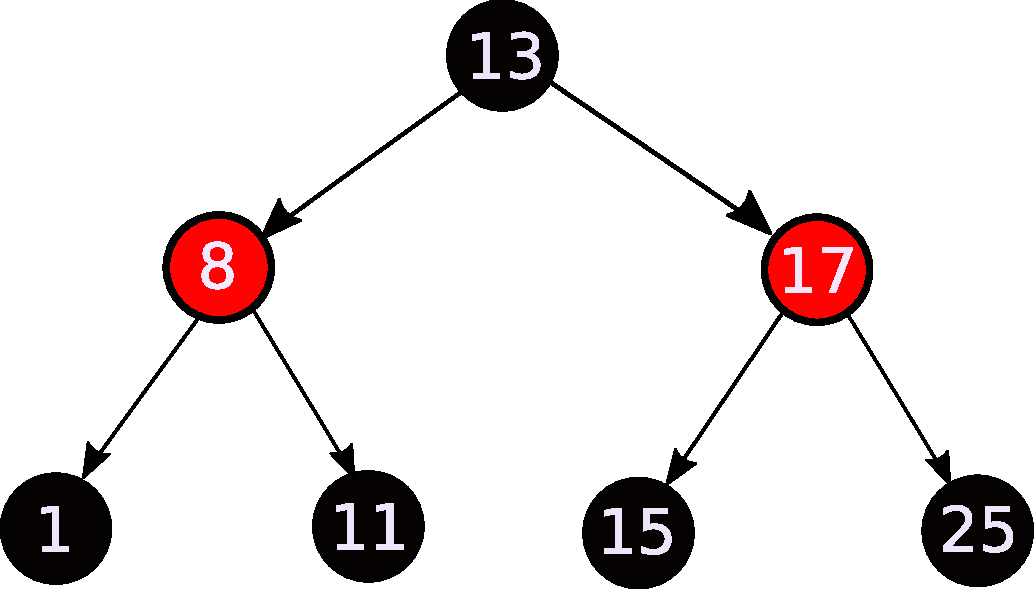
\includegraphics[scale=0.35]{RBTree.pdf}
        \caption{Example of red-black tree with integers}
        \label{img:RBTree}
      \end{figure}

    \subsection{Hash tables}
        A hash table is a generalization of the simpler notion of an ordinary array
        \cite{Cormen:Algorithms}, and each data value has its own index value.
        It is a data structure in which insertion and search operations are very fast \cite{Tuto:Data}.
        Whenever an element is to be inserted, we compute the hash code of the key passed and
        locate the index using that hash code as an index in the array.
        Each data value is converted into an index of the array, using a hash function.
        This is how searching is carried out on Hash tables. The hash functions has to
        do an uniform distribution of keys: each key is equally likely to hash to any of
        the slots of the array, independently of where any other key has hashed to \cite{Cormen:Algorithms}.

        Figure \ref{img:Hash} shows an example of a Hash table.
        \begin{figure}
          \centering
          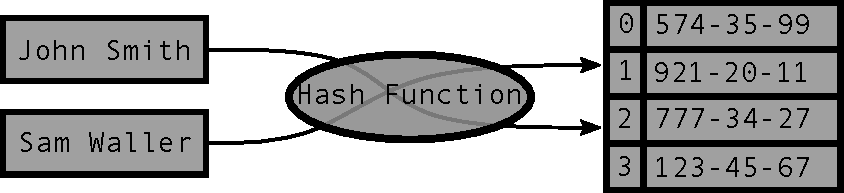
\includegraphics[scale=0.57]{Hash.pdf}
          \caption{Example of Hash table with string keys.}
          \label{img:Hash}
        \end{figure}

    \subsection{B-Trees}
      The B-tree aims to solve the problem of given a large collection of objects, each having a key and an
      value, design a disk-based index structure which efficently supports query and update. It is defined as a tree
      structure which satisfies the following properties:
      \begin{itemize}
        \item A node x has a value $x.num$ as the number of objects stored in x; they are stored in increased order.
        \item Every leaf node has the same depth.
        \item An index node x stores $x.num+1$ child pointers.
        \item Every node except the root node has to be at least half full.
        \item If the root node is an index node, it must have at least two children.
      \end{itemize}
      Figure \ref{img:BTree} shows an example of a B-Tree.
      \begin{figure}[b]
        \centering
        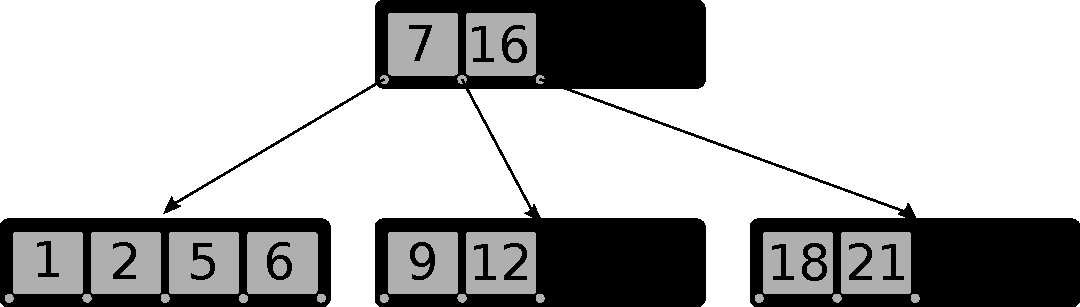
\includegraphics[scale=0.45]{BTree.pdf}
        \caption{Example of B-Tree with integers}
        \label{img:BTree}
      \end{figure}
      The algorithm makes sure that root node is not currenty full and, if it isn't, it inserts it in that node in a sorted
      way. If the root node is full, the algorithm will split it into two nodes and, the previous will pass to a higher level and,
      repeat the process until the node is avaible.

    \subsection{Skip list}
      Let $S_{0}$, $S_{1}$... $S_r$ be a collection of sets that satifies that for the set $S_r = 0$ and for each $i<j$, $0\leq i \leq r$ and $0\leq j\leq r$ then
      $S_j$ is a subset of $S_i$. The index of each set is said to represent the level of each element in the set. Then, a skip list
      is the linked lists $L_i$ each of them containing the respective $S_i$; in every linked list we attach the special keys negative
      and positive infinity at the start and end of the list respectively. Every list will have:
      \begin{itemize}
        \item Horizontal pointers: pointers that connect items in the same list.
        \item Descent pointers: is the pointer that every key k in $L_i$ will have directed to the key k in $L_{i-1}$.
      \end{itemize}
      Figure \ref{img:skipList} shows an example of a skip list.
      To insert an element to a skip list we first begin by marking the skip list (to know how to mark it check the chapter on
      the bibliography) with respect to the x to be inserted. It pushes the marked boxes to a stack when they are
      marked in the procedure and then pop marked boxes from the stack as needed and then insert x next to each of the popped
      boxes.
      The idea of adding the negative and positive infinity is just to put some fixed values of the least and greatest
      value. So, in this way, this concept could apply in other areas as adresses in sorted way and so fourth \cite{Mehta:Handbook}.
      \begin{figure}[t]
        \centering
        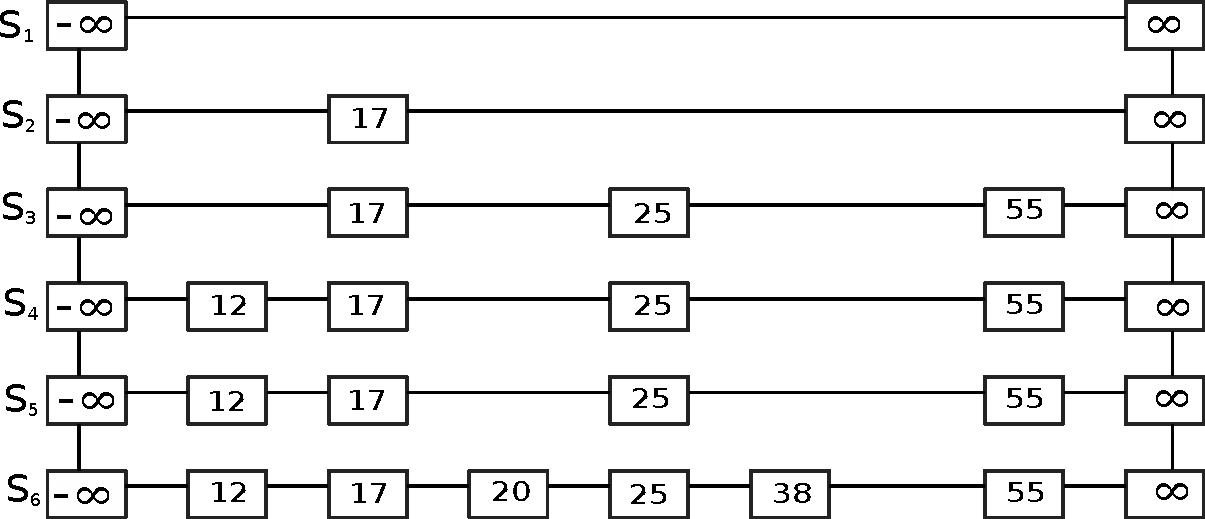
\includegraphics[scale=0.4]{SkipList.pdf}
        \caption{Example of a SkipList}
        \label{img:skipList}
      \end{figure}

  \section{Nash table}
  \begin{figure*}[t]
    \centering
    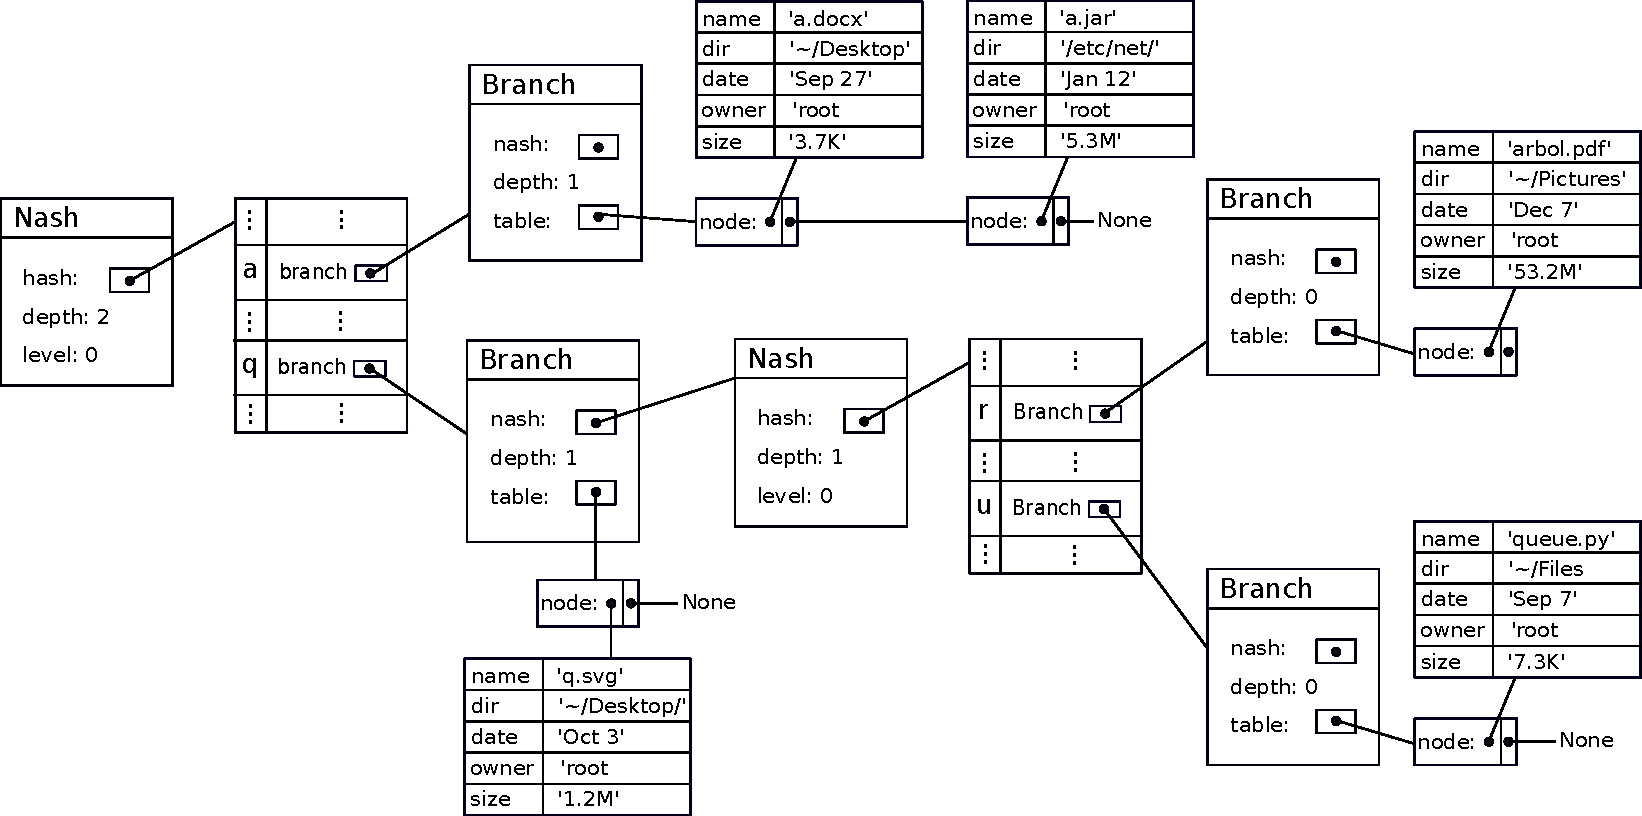
\includegraphics[scale=0.4]{NashTable.pdf}
    \caption{Example of NashTable}
    \label{img:nashT}
  \end{figure*}

  \subsection{Operations of the data structure}

  \subsection{Design criteria of the data structure}
    The NashTable is based on hash tables and double linked lists; searching files
    is the priority. Each NashTable has a hash table, its hash function is associated with the
    nth letter of the name of the file, and n depends on the depth of the structure;
    the hash table has a reference to a Branch with has another NashTable and so fourth.
    This first approach to solve the problem is not optimized for low memory consumption; 



  \bibliographystyle{abbrv}
  \bibliography{sigproc}

\end{document}
